\section{C++ Quick Start}

\subsection{C++ vs C: Key Differences}

% 本页展示 C++ 的所有运算符
\begin{frame}[fragile]{C++ Operators and Keywords (From \textcolor{blue}{\href{https://en.cppreference.com/w/cpp/language/}{cppreference.com}})}
    \begin{columns}
        \begin{column}{0.6\textwidth}
    \begin{figure}
        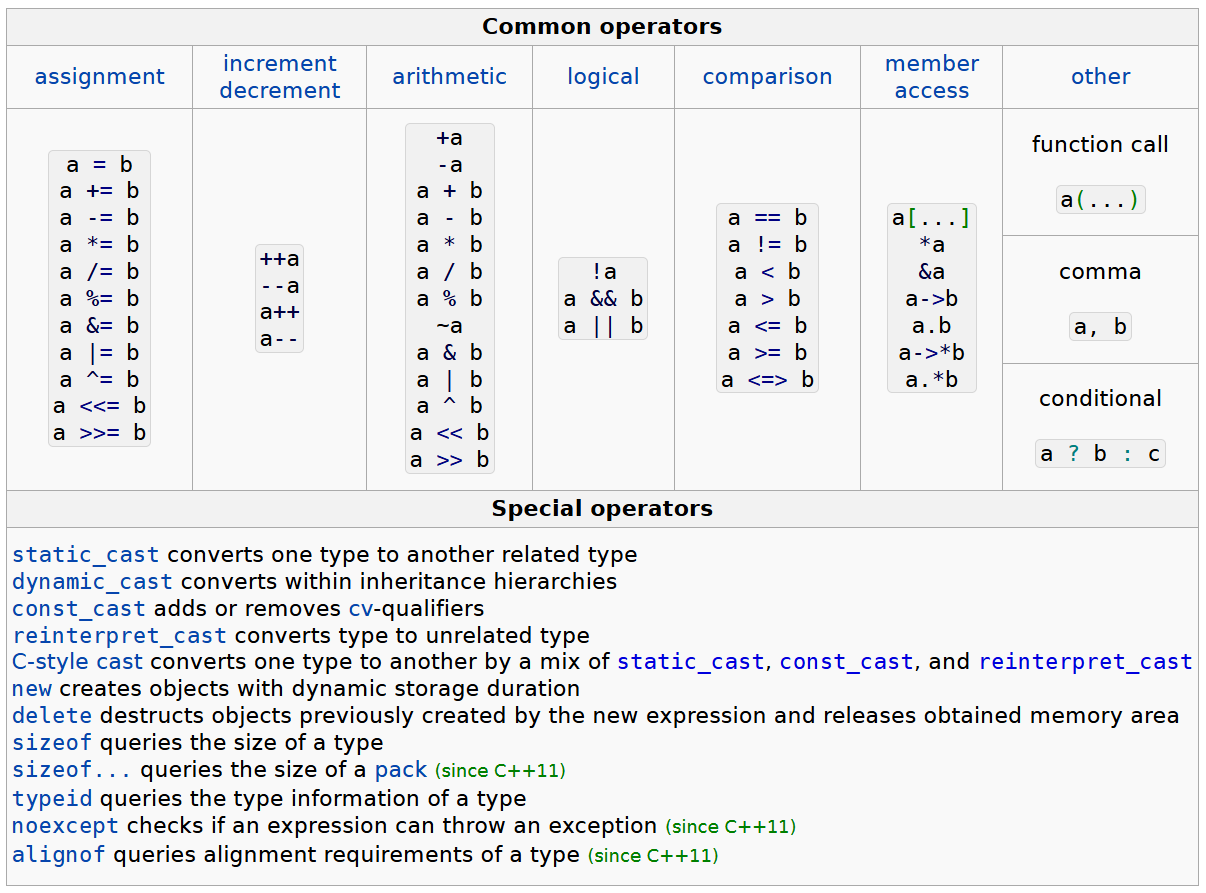
\includegraphics[width=\textwidth]{day8_pm/img/1-operators}
    \end{figure}
        \end{column}
        \begin{column}{0.4\textwidth}
            \begin{figure}
                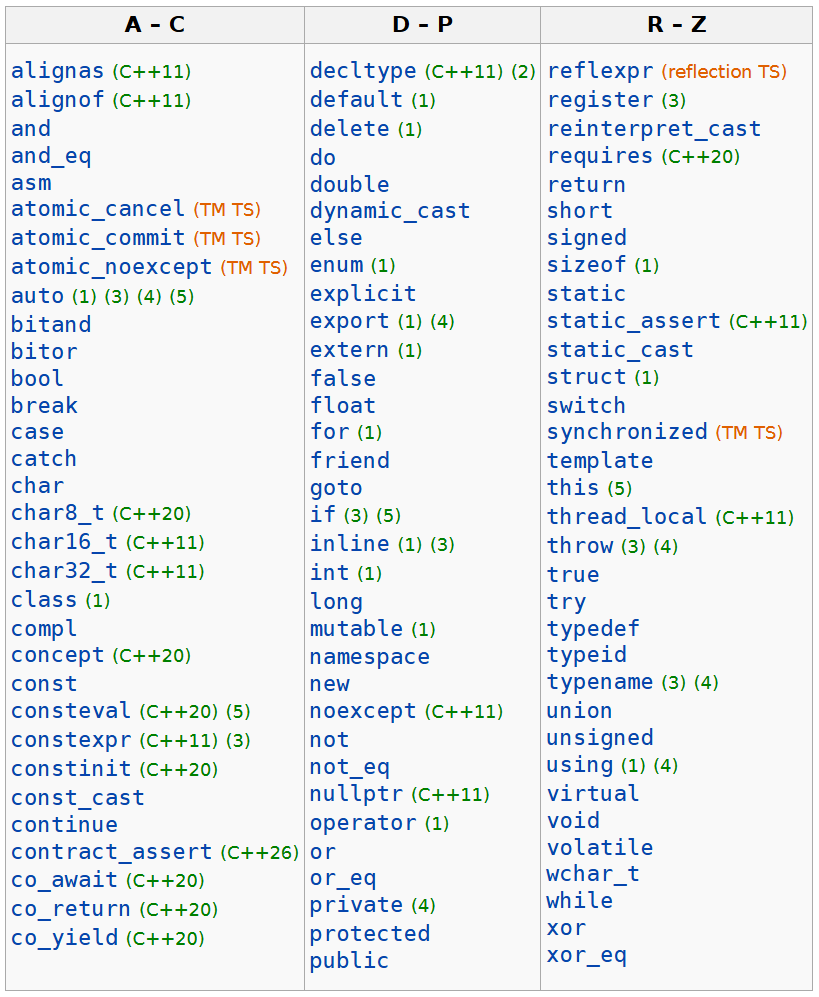
\includegraphics[width=0.9\textwidth]{day8_pm/img/1-keywords}
            \end{figure}
        \end{column}
    \end{columns}
\end{frame}

\begin{frame}[fragile]{\emoji{gear} C++ Operators and Keywords}
    We'll meet some new friends in this class:
    \begin{itemize}
        \item \textbf{I/O}:  \texttt{>>}, \texttt{<<}
        \item \textbf{Memory}: \texttt{new}, \texttt{delete}, \texttt{new[]}, \texttt{delete[]}
        \item \textbf{Type System}: \texttt{auto}, \texttt{decltype}, \texttt{using}, \texttt{operator}
        \item \textbf{Class}: \texttt{::}, \texttt{public}, \texttt{private}, \texttt{protected}, \texttt{friend}, \texttt{virtual}, \texttt{override}, \texttt{final}
    \end{itemize}
\end{frame}

\begin{frame}[fragile]{\emoji{gear} C Standard I/O vs I/O Streams}
	\begin{columns}
		\begin{column}{0.5\textwidth}
			\textbf{C Style}
			\begin{minted}{c}
#include <stdio.h>
#include <stdlib.h>

void print_msg(void) {
    printf("Hello from C!\n");
}

int main() {
    FILE* fp = fopen("test.txt", "r");
    if (fp) {
        // Manual resource management
        char line[100];
        while (fgets(line, 100, fp) != NULL) {
            printf("%s", line);
        }
        fclose(fp);
    }
    return 0;
}
			\end{minted}
		\end{column}
		\begin{column}{0.5\textwidth}
			\textbf{C++ Style}
			\begin{minted}{cpp}
#include <iostream>
#include <fstream>

void print_msg() {
    std::cout << "Hello from C++!" << std::endl;
}

int main() {
    std::ifstream file("test.txt");
    if (file.is_open()) {
        // Automatic resource management
        std::string line;
        while (std::getline(file, line)) {
            std::cout << line << std::endl;
        }
    }
    return 0;
}
			\end{minted}
		\end{column}
	\end{columns}
\end{frame}

% 上页给出代码对比,本页给出讲解
\begin{frame}[fragile]{\emoji{gear} C Standard I/O vs I/O Streams}
    \begin{itemize}
        \item \textbf{C Standard I/O}:
            \begin{itemize}
                \item Uses functions like \texttt{printf}, \texttt{fopen}, and \texttt{fclose}
                \item Requires manual resource management
            \end{itemize}
        \item \textbf{C++ I/O Streams}:
            \begin{itemize}
                \item Uses \textbf{classes} like \texttt{std::ifstream}, and \texttt{std::ofstream}
                \item Automatically manages resources
                \item \textbf{Stream Operators}: \texttt{<<} and \texttt{>>}
            \end{itemize}
    \end{itemize}
    \vspace{0.5em}
    \textbf{Benefits of C++ Streams:}
    \begin{itemize}
        \item Type safety and flexibility
        \item Easier to read and maintain code
        \item Automatic resource cleanup when objects go out of scope
    \end{itemize}
\end{frame}

% 介绍命名空间,标准库的所有名字都在命名空间 std 中
\begin{frame}[fragile]{\emoji{gear} Namespaces}
    \textbf{Namespaces}:
    \begin{itemize}
        \item C++ uses namespaces to avoid \textbf{name collisions}
        \item \textbf{Standard library} functions and classes are in the \texttt{std} namespace
        \item Use \texttt{using namespace std;} to avoid prefixing with \texttt{std::} (should be avoided in header files and large projects)
    \end{itemize}
    \textbf{Example:}
    \begin{minted}[fontsize=\scriptsize]{cpp}
#include <iostream>
using namespace std;
cout << "Hello, World!" << endl;
        \end{minted}
\end{frame}

% 介绍运算符语法
\begin{frame}[fragile]{\emoji{gear} C++ Operators}
    \textbf{Operators in C++}:
    \begin{itemize}
        \item Operators are \textbf{special functions} with concise syntax
        \item Can be \textbf{overloaded} to provide custom behavior for user-defined types
        \item Operators for \textbf{primitive types} like \texttt{int}, \texttt{float}, etc. cannot be overloaded
    \end{itemize}

    \textbf{Overloading Syntax:}
    \begin{minted}[fontsize=\scriptsize]{cpp}
<return_type> operator<operator_symbol>(<parameters>) { /* Implementation */ }
// An illustration of overloading the + operator
int operator+(int a, int b) { return a + b; }
    \end{minted}
\end{frame}

% 介绍 I/O 操作符
\begin{frame}[fragile]{\emoji{gear} I/O Operators}
    \textbf{Signature of I/O Operators}:
    \begin{minted}[fontsize=\scriptsize]{cpp}
template< class Traits >
basic_ostream<char, Traits>&
    operator<<( basic_ostream<char, Traits>& os, const char* s );
basic_istream& operator>>( int& value );
    \end{minted}
    \textbf{Example Usage}:
    \begin{minted}[fontsize=\scriptsize]{cpp}
cout << "Hello, World!" << endl;
cin >> user_input;
    \end{minted}
\end{frame}

% 介绍 C++ 的引用和指针
\begin{frame}[fragile]{\emoji{link} References vs Pointers}
	\begin{columns}
		\begin{column}{0.5\textwidth}
			\textbf{C Pointers}
			\begin{minted}{c}
void swap_c(int* a, int* b) {
    int temp = *a;
    *a = *b;
    *b = temp;
}
int main() {
    int x = 5, y = 10;
    swap_c(&x, &y);  // Pass addresses
    printf("x=%d, y=%d\n", x, y);
    return 0;
}
			\end{minted}
		\end{column}
		\begin{column}{0.5\textwidth}
			\textbf{C++ References}
			\begin{minted}{cpp}
void swap_cpp(int& a, int& b) {
    int temp = a;
    a = b;
    b = temp;
}
int main() {
    int x = 5, y = 10;
    swap_cpp(x, y);  // Direct pass
    cout << "x=" << x << ", y=" << y << endl;
    return 0;
}
			\end{minted}
		\end{column}
	\end{columns}

	\vspace{0.5em}
	\begin{itemize}
        \item References are \textbf{aliases} for existing objects: \texttt{int a; int\& b = a;}
		\item References must be initialized and cannot be reassigned
	\end{itemize}
\end{frame}

\subsection{Object-Oriented Programming}
\begin{frame}[fragile]{\emoji{gear} What is Object-Oriented Programming?}
    \textbf{Think of it like building with LEGO blocks:}
    \begin{itemize}
        \item In C: You have \textbf{functions} (tools) and \textbf{variables} (materials)
        \item In C++: You can create \textbf{custom LEGO blocks} (classes) that contain both data and functions
    \end{itemize}

    \vspace{0.5em}
    \textbf{C++ OOP Features:}
    \begin{itemize}
        \item \textbf{Classes and Objects}: Define custom data types with behavior
        \item \textbf{Encapsulation}: Keep data safe inside the "block"
        \item \textbf{Inheritance}: Create new blocks based on existing ones
        \item \textbf{Polymorphism}: Use different blocks with the same interface
    \end{itemize}
\end{frame}

\begin{frame}[fragile]{\emoji{building-construction} Classes vs Structs: From C to C++}
	\begin{columns}
		\begin{column}{0.5\textwidth}
			\textbf{C Struct (Data Only)}
			\begin{minted}{c}
struct Student {
    char name[50];
    int age;
    float gpa;
};
void print_student(struct Student s) {
    printf("Name: %s\n", s.name);
    printf("Age: %d\n", s.age);
    printf("GPA: %.2f\n", s.gpa);
}
int main() {
    struct Student alice = {"Alice", 20, 3.8};
    print_student(alice);
    return 0;
}
			\end{minted}
		\end{column}
		\begin{column}{0.5\textwidth}
			\textbf{C++ Class (Data + Functions)}
			\begin{minted}{cpp}
class Student {
private:
    string name;
    int age;
    float gpa;
public:
    Student(string n, int a, float g)
        : name(n), age(a), gpa(g) {}
    void print() {
        cout << "Name: " << name << endl;
        cout << "Age: " << age << endl;
        cout << "GPA: " << gpa << endl;
    }
};
int main() {
    Student alice("Alice", 20, 3.8);
    alice.print();  // Object calls its own method
    return 0;
}
			\end{minted}
		\end{column}
	\end{columns}
\end{frame}

\begin{frame}[fragile]{\emoji{lock} Encapsulation: Protecting Your Data}
    \textbf{Why Encapsulation?}
    \begin{itemize}
        \item \textbf{Data Protection}: Prevent accidental modification
        \item \textbf{Interface Control}: Define how others can use your class
        \item \textbf{Easy Maintenance}: Change implementation without breaking user code
    \end{itemize}
\end{frame}

\begin{frame}[fragile]{\emoji{lock} Encapsulation: Protecting Your Data}
    \textbf{Access Levels:}
    \begin{minted}[fontsize=\scriptsize]{cpp}
class BankAccount {
private:    // Only this class can access
    double balance;

public:     // Anyone can access
    void deposit(double amount) {
        if (amount > 0) balance += amount;  // Safe deposit
    }

    double getBalance() const { return balance; }  // Read-only access

protected:  // This class and its children can access
    void setBalance(double newBalance) { balance = newBalance; }
};
    \end{minted}
\end{frame}

\begin{frame}[fragile]{\emoji{family} Inheritance: Building on Existing Code}
    \textbf{Like a Family Tree:} Children inherit traits from parents

    \begin{columns}
        \begin{column}{0.3\textwidth}
            \textbf{Base Class (Parent)}
    \begin{minted}{cpp}
class Animal {
protected:
    string name;
public:
    Animal(string n) : name(n) {}
    void eat() { cout << name << " is eating\n"; }
    virtual void makeSound() { cout << name << " makes a sound\n"; }
};
    \end{minted}
        \end{column}
        \begin{column}{0.7\textwidth}
            \textbf{Derived Class (Child)}
    \begin{minted}{cpp}
class Dog : public Animal {
public:
    Dog(string n) : Animal(n) {}  // Call parent constructor
    void makeSound() override {        // Override parent method
        cout << name << " barks: Woof!\n";
    }
    void wagTail() { cout << name << " wags tail\n"; }  // New method
};

int main() {
    Dog buddy("Buddy");
    buddy.eat();        // Inherited from Animal
    buddy.makeSound();  // Dog's own version
    buddy.wagTail();    // Dog-specific behavior
    return 0;
}
    \end{minted}
        \end{column}
    \end{columns}
\end{frame}

\begin{frame}[fragile]{\emoji{shuffle-tracks-button} Polymorphism: One Interface, Many Forms}
    \textbf{Like a Universal Remote:} Same buttons, different devices

    \begin{columns}
        \begin{column}{0.6\textwidth}
    \begin{minted}{cpp}
class Shape {
public:
    virtual double area() = 0;  // Pure virtual function
    virtual ~Shape() = default;
};
class Circle : public Shape {
    double radius;
public:
    Circle(double r) : radius(r) {}
    double area() override { return 3.14159 * radius * radius; }
};
class Rectangle : public Shape {
    double width, height;
public:
    Rectangle(double w, double h) : width(w), height(h) {}
    double area() override { return width * height; }
};
    \end{minted}
        \end{column}
        \begin{column}{0.4\textwidth}

    \begin{minted}{cpp}
vector<unique_ptr<Shape>> shapes;
shapes.push_back(make_unique<Circle>(5.0));
shapes.push_back(
    make_unique<Rectangle>(4.0, 6.0));
for (auto& shape : shapes) {
    cout << "Area: " << shape->area()
         << endl;
    // Calls correct method
}
    \end{minted}
    \end{column}
    \end{columns}
\end{frame}

\subsection{Containers and Algorithms}
\begin{frame}[fragile]{\emoji{toolbox} STL: Your Programming Toolbox}
    \textbf{Standard Template Library (STL):}
    \begin{itemize}
        \item \textbf{Containers}: Ready-made data structures (like toolboxes)
        \item \textbf{Algorithms}: Common operations (like tools)
        \item \textbf{Iterators}: Ways to access container elements (like handles)
    \end{itemize}

    \vspace{0.5em}
    \textbf{Why use STL instead of arrays?}
    \begin{itemize}
        \item \textbf{Safety}: Automatic bounds checking and memory management
        \item \textbf{Convenience}: Built-in functions for common operations
        \item \textbf{Performance}: Optimized implementations
        \item \textbf{Compatibility}: Works seamlessly with C++ features
    \end{itemize}
\end{frame}

\begin{frame}[fragile]{\emoji{package} Common Containers: Your Data Storage Options}
	\begin{columns}
		\begin{column}{0.5\textwidth}
			\textbf{Vector: Dynamic Array}
			\begin{minted}{cpp}
vector<int> numbers;
// Add elements
numbers.push_back(10);
numbers.push_back(20);
numbers.push_back(30);
// Access elements
cout << "First: " << numbers[0] << endl;
cout << "Size: " << numbers.size() << endl;
// Iterate through all
for (int num : numbers) { cout << num << " "; }
			\end{minted}
		\end{column}
		\begin{column}{0.5\textwidth}
			\textbf{Map: Key-Value Storage}
			\begin{minted}{cpp}
map<string, int> scores;
// Add key-value pairs
scores["Alice"] = 95;
scores["Bob"] = 87;
scores["Charlie"] = 92;
// Look up values
cout << "Alice's score: "
            << scores["Alice"] << endl;
// Check if key exists
if (scores.find("David") != scores.end()) {
    cout << "David found\n";
} else {
    cout << "David not found\n";
}
			\end{minted}
		\end{column}
	\end{columns}
\end{frame}

\begin{frame}[fragile]{\emoji{gear} Algorithms: Ready-Made Solutions}
    \textbf{Common algorithms you'll use:}
    \begin{table}[]
        \begin{tabular}{|l|l|}
        \hline
        \textbf{Category}       & \textbf{Algorithms}                                                                 \\ \hline
        \textbf{Sorting}        & \texttt{sort}, \texttt{stable\_sort}, \texttt{partial\_sort}, \texttt{nth\_element} \\ \hline
        \textbf{Searching}      & \texttt{find}, \texttt{binary\_search}, \texttt{lower\_bound}, \texttt{upper\_bound} \\ \hline
        \textbf{Modifying}      & \texttt{copy}, \texttt{swap}, \texttt{replace}, \texttt{fill}, \texttt{transform}   \\ \hline
        \textbf{Set Operations} & \texttt{set\_union}, \texttt{set\_intersection}, \texttt{set\_difference}           \\ \hline
        \textbf{Numeric}        & \texttt{accumulate}, \texttt{inner\_product}, \texttt{adjacent\_difference}         \\ \hline
        \end{tabular}
    \end{table}
\end{frame}

\begin{frame}[fragile]{\emoji{gear} Algorithms: Ready-Made Solutions}
    \begin{minted}[fontsize=\scriptsize]{cpp}
vector<int> numbers = {64, 34, 25, 12, 22, 11, 90};
// Sort the vector
sort(numbers.begin(), numbers.end());
cout << "Sorted: ";
for (int n : numbers) cout << n << " ";
cout << endl;
// Find an element
auto it = find(numbers.begin(), numbers.end(), 25);
if (it != numbers.end()) {
    cout << "Found 25 at position: "
                << (it - numbers.begin()) << endl;
}
// Count elements greater than 30
int count = count_if(numbers.begin(), numbers.end(),
    [](int n) { return n > 30; });
cout << "Numbers > 30: " << count << endl;
    \end{minted}
\end{frame}

\begin{frame}[fragile]{\emoji{person-tipping-hand} More on STL Algorithms}
    \begin{figure}
        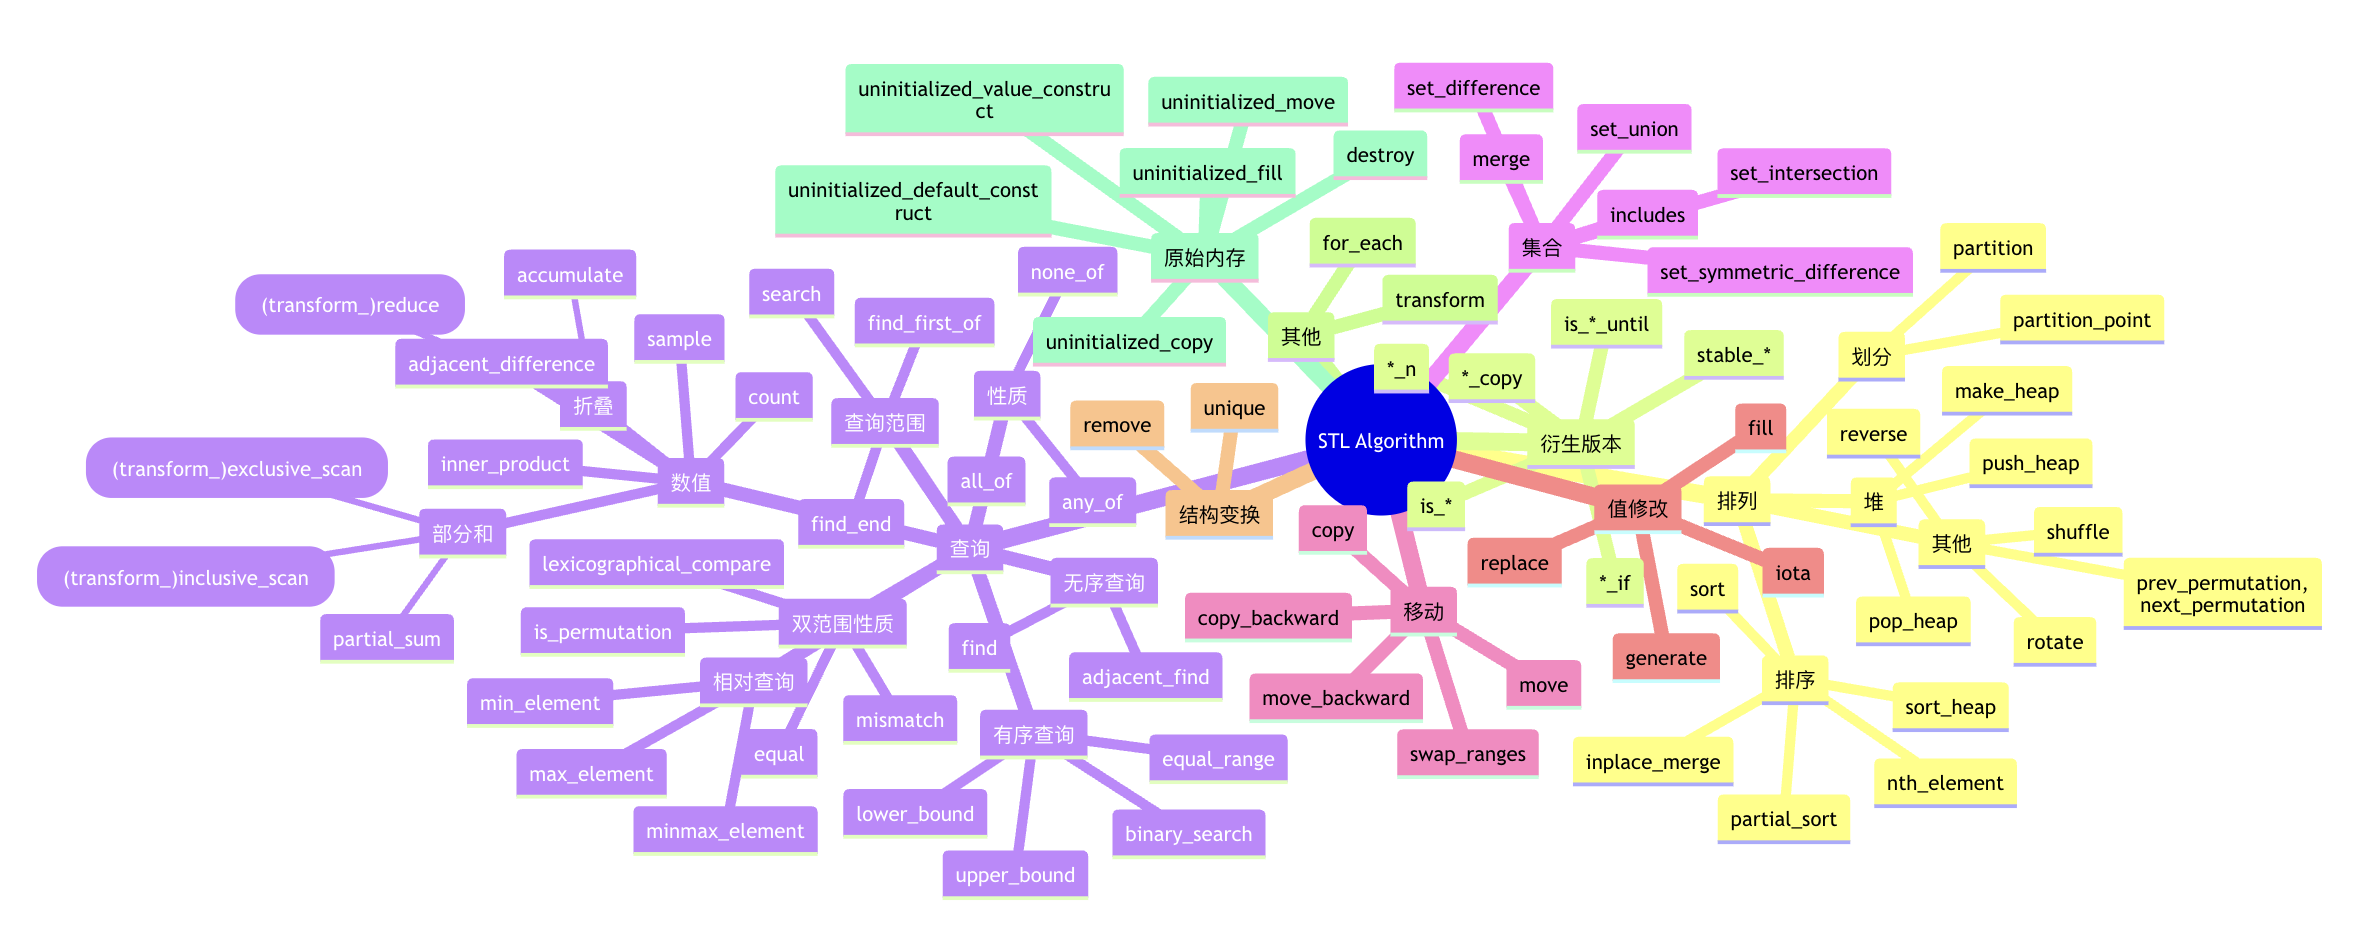
\includegraphics[width=\textwidth]{day8_pm/img/2-algorithms}
    \end{figure}
\end{frame}

\begin{frame}[fragile]{\emoji{person-tipping-hand} More on STL Algorithms}
    \textcolor{blue}{\href{https://www.youtube.com/watch?v=2olsGf6JIkU&ab_channel=CppCon}{CppCon 2018: 105 STL Algorithms in Less Than an Hour}}
    \begin{figure}
        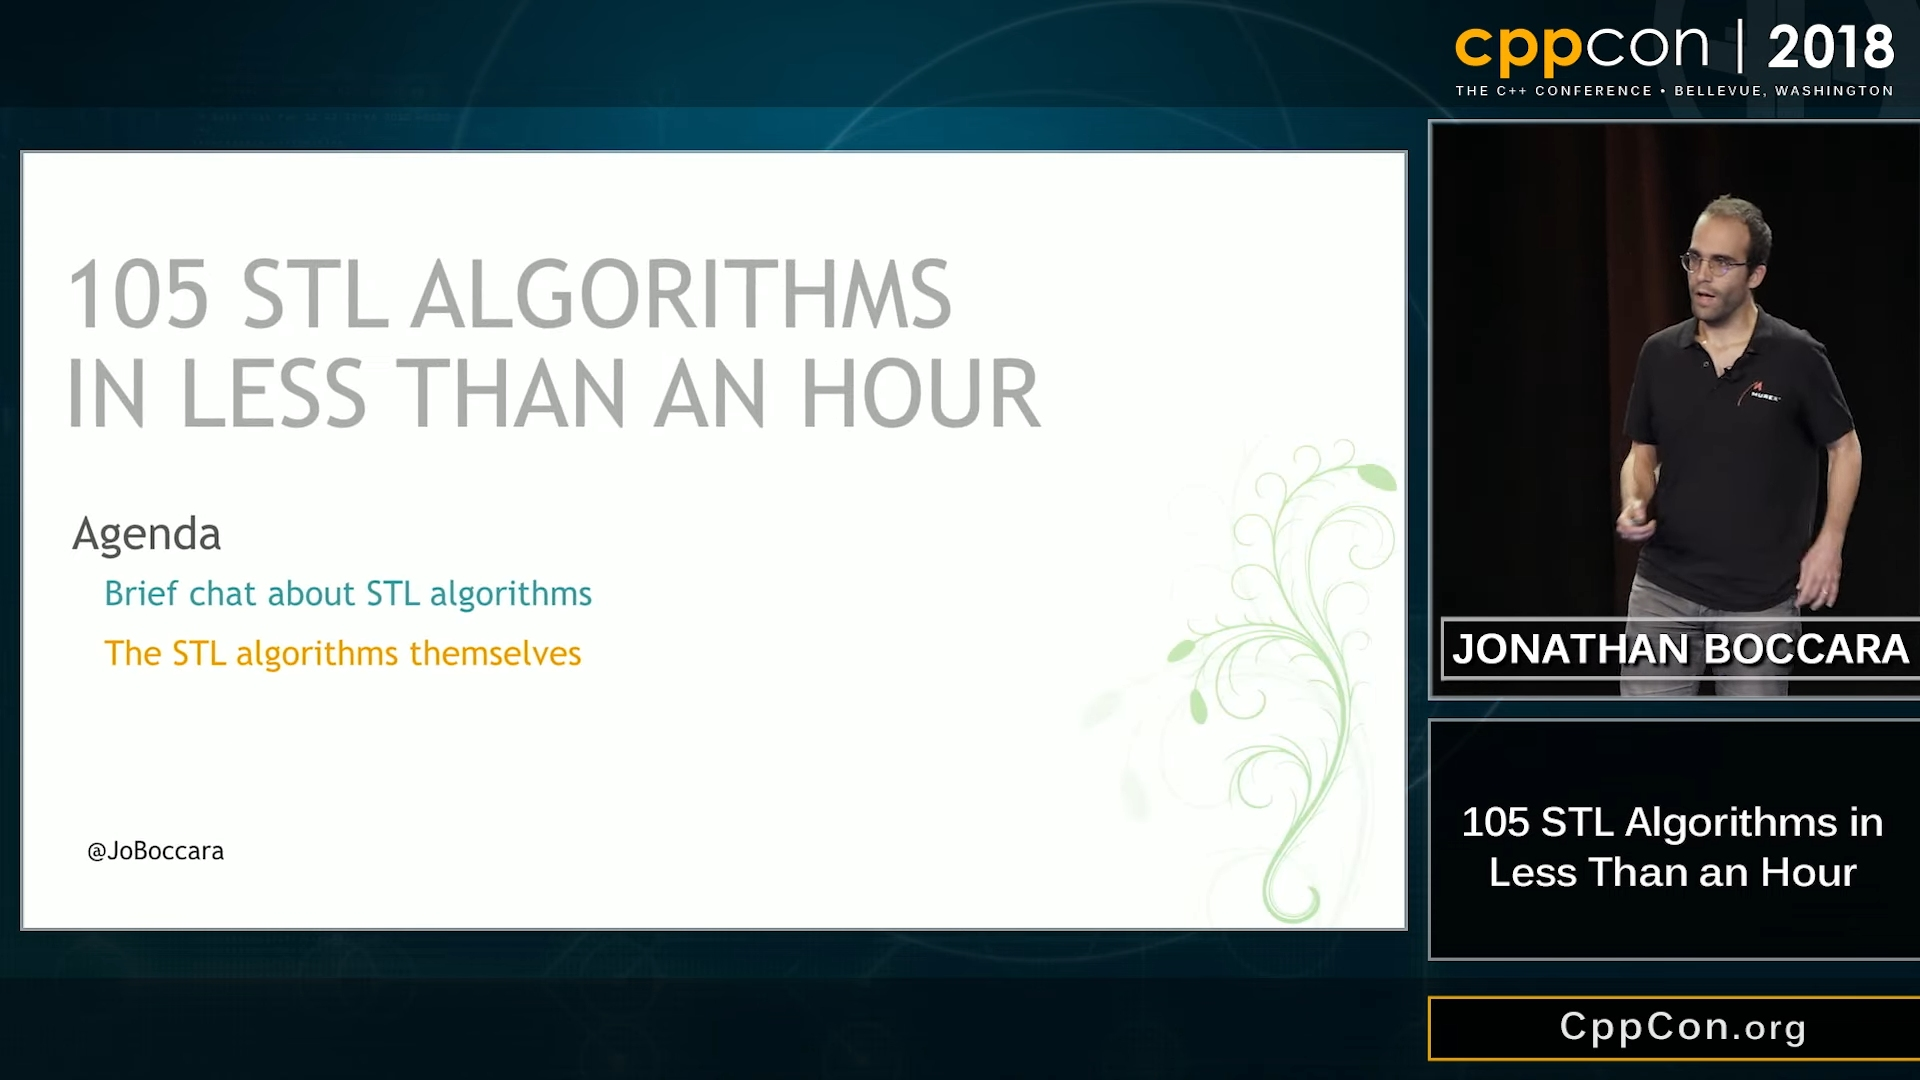
\includegraphics[width=0.7\textwidth]{day8_pm/img/2-cppcon2018}
    \end{figure}
\end{frame}

\begin{frame}[fragile]{\emoji{vs} Containers vs C Arrays: The Upgrade}
	\begin{columns}
		\begin{column}{0.5\textwidth}
			\textbf{C Arrays (Manual Everything)}
			\begin{minted}{c}
int arr[] = {1, 3, 2};
int size = 0;
// must write your compare function
qsort(ints, size, sizeof(int), compare_ints);
for (int i = 0; i < size; i++) {
    printf("%d ", arr[i]);
}
			\end{minted}
		\end{column}
		\begin{column}{0.5\textwidth}
			\textbf{C++ Containers (Automatic)}
			\begin{minted}{cpp}
// Dynamic size, automatic memory
vector<int> arr = {1, 3, 2};
sort(arr.begin(), arr.end());
for (int num : arr) {
    cout << num << " ";
}
			\end{minted}
		\end{column}
	\end{columns}

	\vspace{0.5em}
	\textbf{Benefits:} Safer, shorter, and often faster code!
\end{frame}

\subsection{Essential Features for Concurrency}
\begin{frame}[fragile]{\emoji{rocket} Lambda Expressions: The Core of Thread Functions}
	\begin{columns}
		\begin{column}{0.5\textwidth}
			\textbf{C Function Pointers}
			\begin{minted}{c}
#include <pthread.h>

void* thread_func(void* arg) {
    int id = *(int*)arg;
    printf("Thread %d running\n", id);
    return NULL;
}

int main() {
    pthread_t thread;
    int id = 1;
    pthread_create(&thread, NULL,
                   thread_func, &id);
    pthread_join(thread, NULL);
    return 0;
}
			\end{minted}
		\end{column}
		\begin{column}{0.5\textwidth}
			\textbf{C++ Lambda}
			\begin{minted}{cpp}
#include <thread>
#include <iostream>

int main() {
    int id = 1;

    // Lambda expression
    auto thread_func = [id]() {
        cout << "Thread " << id
                  << " running" << endl;
    };

    thread t(thread_func);
    t.join();

    return 0;
}
			\end{minted}
		\end{column}
	\end{columns}

\end{frame}

\begin{frame}[fragile]{\emoji{brain} Lambda Expressions: The Core of Thread Functions}
	\textbf{Lambda Capture Modes:}
	\begin{itemize}
		\item \texttt{[]} - Capture nothing
		\item \texttt{[=]} - Capture by value
		\item \texttt{[\&]} - Capture by reference
		\item \texttt{[id]} - Capture specific variable by value
	\end{itemize}
\end{frame}

\begin{frame}[fragile]{\emoji{brain} Smart Pointers vs Manual Memory Management}
	\begin{columns}
		\begin{column}{0.5\textwidth}
			\textbf{C malloc/free}
			\begin{minted}[fontsize=\tiny]{c}
typedef struct {
    int data;
} Resource;
// Manual allocation
Resource* ptr = malloc(sizeof(Resource));
if (!ptr) return -1;
ptr->data = 42;
printf("Data: %d\n", ptr->data);
// Must remember to free
free(ptr);
// ptr is now dangling!
			\end{minted}
		\end{column}
		\begin{column}{0.5\textwidth}
			\textbf{C++ new/delete}
			\begin{minted}[fontsize=\tiny]{cpp}
class Resource {
    int data;
};
// Manual allocation
Resource* ptr = new Resource(42);
cout << "Data: " << ptr->getData() << endl;
// Must remember to delete
delete ptr;
// ptr is now dangling!
			\end{minted}
			\textbf{C++ Smart Pointers}
			\begin{minted}[fontsize=\tiny]{cpp}
// Automatic memory management
auto ptr = make_unique<Resource>(42);
cout << "Data: " << ptr->getData() << endl;
// Automatic cleanup when out of scope
// No manual delete needed!
			\end{minted}
		\end{column}
	\end{columns}

	\vspace{0.5em}
	\textbf{Benefits of Smart Pointers:}
	\begin{itemize}
		\item \textbf{Automatic cleanup}: No memory leaks
		\item \textbf{Exception safety}: Cleanup even when exceptions occur
		\item \textbf{Clear ownership}: \texttt{unique\_ptr} vs \texttt{shared\_ptr}
	\end{itemize}
\end{frame}

\begin{frame}[fragile]{\emoji{brain} Auto Type Deduction: Let the Compiler Figure It Out}
	\begin{columns}
		\begin{column}{0.5\textwidth}
			\textbf{Without Auto (Verbose)}
			\begin{minted}{cpp}
int x = 42;
double y = 3.14;
const char* str = "Hello";

vector<int> vec{1,2,3};
vector<int>::iterator it = vec.begin();

// Very long type names
map<string, int> scores;
map<string, int>::iterator map_it
    = scores.find("Alice");
			\end{minted}
		\end{column}
		\begin{column}{0.5\textwidth}
			\textbf{With Auto (Clean)}
			\begin{minted}{cpp}
auto x = 42;              // int
auto y = 3.14;            // double
auto str = "Hello";       // const char*
vector<int> vec{1,2,3};
auto it = vec.begin();    // vector<int>::iterator
// Complex types made simple
map<string, int> scores;
auto map_it = scores.find("Alice");
// Range-based for loop
for(auto& pair : scores) {
    cout << pair.first << ": " << pair.second << endl;
}
			\end{minted}
		\end{column}
	\end{columns}

	\vspace{0.5em}
	\textbf{Benefits:}
	\begin{itemize}
		\item \textbf{Less typing}: Compiler deduces the type
		\item \textbf{Maintainable}: Change type in one place
		\item \textbf{Generic}: Works with complex template types
	\end{itemize}
\end{frame}
